\documentclass[openany,12pt]{memoir}
\usepackage[utf8]{inputenc} 
\usepackage[czech]{babel}
\usepackage[T1]{fontenc}
\usepackage[top=1.5cm, bottom=2cm, left=2cm, right=2cm]{geometry}  % --> NASTAVENÍ OKRAJŮ
\usepackage{fancyhdr}
\usepackage{graphicx}
%\usepackage{xwatermark}
\usepackage{xcolor}
\usepackage{changepage}
\usepackage{pdfpages}
\usepackage{lettrine}
\usepackage{indentfirst}  %Důležité pro formátování
\usepackage[pages=some]{background}
\usepackage{wrapfig}

%%%%%%%%%%%%%%%%%%%%%%%%%%%%%%%%%%%%%%
%  FONT                              %
%%%%%%%%%%%%%%%%%%%%%%%%%%%%%%%%%%%%%%
\usepackage{amssymb}
\usepackage{tgschola}

%%%%%%%%%%%%%%%%%%%%%%%%%%%%%%%%%%%%%%
%  Obrázky v textu                   %
%%%%%%%%%%%%%%%%%%%%%%%%%%%%%%%%%%%%%%
\usepackage{tikz}
%\tikz[remember picture,overlay] \node[opacity=0.3,inner sep=0pt] at (current page.center){\includegraphics[width=\paperwidth,height=\paperheight]{example-image}};
%Tímto příkazem se na následující stránku vloží pozadí. Pokud pozadí uděláme
%tak, aby bylo velikosti a4, bylo prázdné až na malůvku, můžeme takto vkládat
%obrázky.
%Pozn.: kompilovat se musí dvakrát


%%%%%% Package na zpěvník
\usepackage[full]{leadsheets}%http://mirrors.nic.cz/tex-archive/macros/latex/contrib/leadsheets/leadsheets_en.pdf   --> dokumentace	
\definesongtitletemplate{empty}{} 
\setchords{
format = \bfseries \sffamily,   %tučné akordy
minor = {mi},% 
input-notation = {german},%
output-notation = {german}%
}
\definesongtitletemplate{empty}{} 


\newlength{\drop}
% VODOZNAK
%\newwatermark[pages=1-,color=red!50,angle=0,scale=2, xpos=0,ypos=0]{\includegraphics[width=5cm]{obr/pozadi2.jpg}} %--> dvojka na pozadí


%%%%%%%%%%%%%%%%%%%%%%%%%%%%%%%%%%%%%%%%%%%%%%%%%%
%		 Vlastní příkazy
\newcommand{\defaulttabscale}{0.87}
\newcommand{\defaultfretscale}{1.7}

\newcounter{Slokočet}   %Automatické číslování slok
\newcommand{\mezera}{
\phantom{.}

}   %Horizontální odsazení slok (poněkud blbě zadefinovaný, ale jinak se formát rozbije jako wtf prostě)
\newcommand{\stred}{5.2cm}   %%% Na zarovnání slok doprostřed, pozn. automatičtější zarovnávání na střed nejde
\newcommand{\carka}{,\:}
\newcommand{\m}[1]{\color{white}{#1}}  %Pro akordy
\newcommand{\ap}{'}	%Pro apostrof
\newcommand{\elipsa}{\kern\fontdimen3\font} %Příkaz pro lepší zacházení s výpustkami (=...); je to vpodstatě jen mezera mezi tečkama výpustky
\newcommand{\pindent}{17.62482 pt} %Správná velikost \parindentu u layoutu se dvěma minipageama
\newcommand{\predtitle}{\huge}
\newcommand{\mezisloupci}{\phantom{TT}} %Místo mezi dvěma sloupci na jedné stránce
\newcommand{\z}{\hspace*{\fill}\null}

%%% Možné velikosti písem 
\newcommand{\normalni}{\normalsize}
\newcommand{\velky}{\fontsize{14.4}{15}\selectfont}
\newcommand{\vetsi}{\fontsize{15}{16}\selectfont}
\newcommand{\nejvetsi}{\fontsize{16}{17}\selectfont}
\newcommand{\nejnejvetsi}{\fontsize{17}{19}\selectfont}

%%% Stará definice sloky spoléhající na indenty
%\newlength{\pismeno}
%\settowidth{\pismeno}{x} %Tohle není moc ideální velikost, ale funguje
%\newif\ifslokavelka
%\slokavelkafalse
%\newcommand{\sloka}{
%\ifnum \value{Slokočet}>8  %Pokud je sloka dvouciferná
%\mezera \noindent \addtocounter{Slokočet}{1} \hspace*{-\pismeno}\arabic{Slokočet}.
%\else %Pokud jen jednociferná
%\mezera \noindent \addtocounter{Slokočet}{1} \arabic{Slokočet}. 
%\fi
%} 	%sloka, která se automaticky čísluje

\newcommand{\distanc}{\:}  %Vzdálenost čísla sloky před slokou
\newlength{\delkaargumentu}
%%% Sloka s automatickým číslováním
\newcommand{\sloka}{%
\addtocounter{Slokočet}{1}% Zvýší se o 1 počet slok
\mezera%  Sloka se odsadí vertikálně
\settowidth{\delkaargumentu}{\arabic{Slokočet}.\distanc}% Zde se určí délka odsazení 
\hspace*{-\delkaargumentu}%
\arabic{Slokočet}.\distanc%
\ignorespaces% Aby nevznikaly zbytečné mezery
}


%%% Sloka s vlastním argumentem
\newcommand{\ssloka}[1]{%     
\settowidth{\delkaargumentu}{#1\distanc}
\mezera%
\hspace*{-\delkaargumentu}%
#1\distanc%
\ignorespaces%
}  

%%% Refrén
\newcommand{\refren}[1][0]{%  Nepovinný argument sděluje, kolikátý refrén toto je, bez argumentu se vytiskne pouze refrén
\ifnum #1>0 %Pokud nepovinný argument existuje
\mezera%
\settowidth{\delkaargumentu}{\textbf{R$_{\text{#1}}$:}\distanc}%
\hspace*{-\delkaargumentu}%
\textbf{R$_{\text{#1}}$:}\distanc%
\ignorespaces%
\else %Pokud nepovinný argument neexistuje
\mezera%
\settowidth{\delkaargumentu}{\textbf{R:}\distanc}%
\hspace*{-\delkaargumentu}%
\textbf{R:}\distanc%
\ignorespaces%
\fi
}

\newcommand{\predehra}{\ssloka{\textbf{Předehra:}}}

%%% Capo
\newcommand{\kapodastr}[1]{%
\textit{Capo {#1}}
}

\newcommand{\includefret}[1]{\includegraphics[scale=\defaultfretscale]{../Akordy/msc/#1.pdf}}

\addto\captionsczech{\renewcommand{\contentsname}{Seznam písní}}

%%%%%%%%%%%%%%%%%%%%%%%%%%%%%%%%%%%%
%    FORMÁTOVÁNÍ                   %
%%%%%%%%%%%%%%%%%%%%%%%%%%%%%%%%%%%%

%%% Vlevo zarovnaný text s blokem zarovnaným na střed
\usepackage{varwidth}% http://ctan.org/pkg/varwidth
\newenvironment{centerjustified}{%
  \begin{center} % so the minipage is centered
  \begin{varwidth}[t]{\textwidth}	
  \raggedright % so the minipage's text is left justified
  \setlength{\parindent}{\pindent}
}{%
  \end{varwidth}
  \end{center}
}

%%% Pozadí
\newcommand{\pozadi}[1]{
\backgroundsetup{
scale=1,
angle=0,
contents={%
  \includegraphics[width=\paperwidth,height=\paperheight]{#1}
  }%
}
\BgThispage
}


%%% Libovolné posouvání elementů (hlavně se používá na akordy),
%%% přičemž element má dimenze (0,0), takž neovlivní předchozí formátování.
\makeatletter
\newcommand*{\shifttext}[2]{%
  \settowidth{\@tempdima}{#2}%
  \makebox[\@tempdima]{\hspace*{#1}#2}%
}
\makeatother

%\cheatbox{X}{Y}{Element}
\newcommand{\cheatbox}[3]{%
\shifttext{#1}{\raisebox{#2}[0pt][0pt]{%
#3%
}}%
}


%Hlavnička END
\usepackage{hyperref}
\begin{document}
\sffamily %Sans-serif pro lepší čitelnost

\pagestyle{empty}
\newgeometry{top=1.5cm, bottom = 0cm, left = 2cm, right = 2cm}

\newpage

%Pro kompilaci je důležitý, aby ten \input a \end{document} zůstali na posledních
%dvou řádcích!!!!

\velky
\newpage
% PÍSNIČKA

\begin{song}{title=\predtitle\centering Pohádka \\\large Karel Plíhal\vspace*{-1.0cm}}  %% sem se napíše jméno songu a autor
\begin{centerjustified}
\mezera \noindent \textbf{Rec:}
Takhle nějak to bylo: jedlo se, zpívalo, pilo,

princezna zářila štěstím v hotelu nad náměstím,

drak hlídal u dveří sálu, na krku pletenou šálu,

Dědové Vševědi okolo Popelky žvatlavě slibují šaty a kabelky,

každý si odnáší kousíček úsměvu,

dešťový mraky se chystaly ke zpěvu,

hosté se sjíždějí k veliké veselce,

paprsky luceren metají kozelce

a stíny ořechů orvaných dohola

pletou se latícím kočárům pod kola,

Šmudla si přivezl v odřeným wartburgu

kámošku z dětství, prej nějakou Sněhurku,

vrátný se zohýbá pro tučné spropitné

a kdo mu proklouzne, tak toho nechytne,

kouzelník za dvacku vykouzlí pět bonů

a vítr na věži opřel se do zvonů,

„Na zdraví nevěsty, na zdraví ženicha!“,

dvě sousta do kapsy a jednou do břicha,

náhle se za oknem objevil skřítek,

rozhrnul oponu z máminejch kytek,

pěkně se usmál a pěkně se podíval

a pak mi po očku do ucha zazpíval:


\refren
^{G\,\,}Dej mi ruku ^{D{\z}}svou, ^{{\z}Emi}studenou od okenních ^{Hmi/D}skel,

všichni tě ^{C{\z}}mezi sebe ^{Hmi/D}zvou

a ^{C}já jsem ^{D}tu proto, ^{G{\z}}abys ^{{\z}Emi}šel.~


\mezera \noindent \textbf{Rec:}
Na plný obrátky letíme světem,

všechny ty pohádky patřily dětem,

dneska už se neplatí buchtama za skutky,

sudičky sesmolí kádrový posudky,

obložen prošlými dlužními úpisy,

koukám se z okna a vzpomínám na kdysi,

jak se mi za oknem objevil skřítek,

rozhrnul oponu z máminejch kytek,

pěkně se usmál a pěkně se podíval

a pak mi po očku do ucha zazpíval:

\refren $2\times$

\hspace*{-1.5cm}
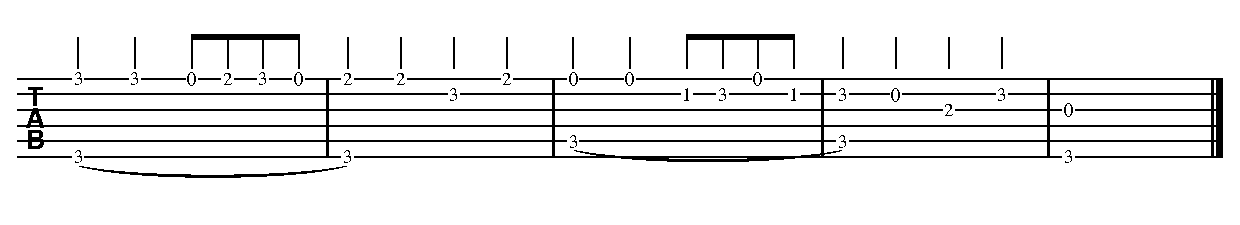
\includegraphics[scale=0.83]{../taby/pohadka.pdf}
\hspace*{-1.5cm}
\end{centerjustified}

\newpage
\centering
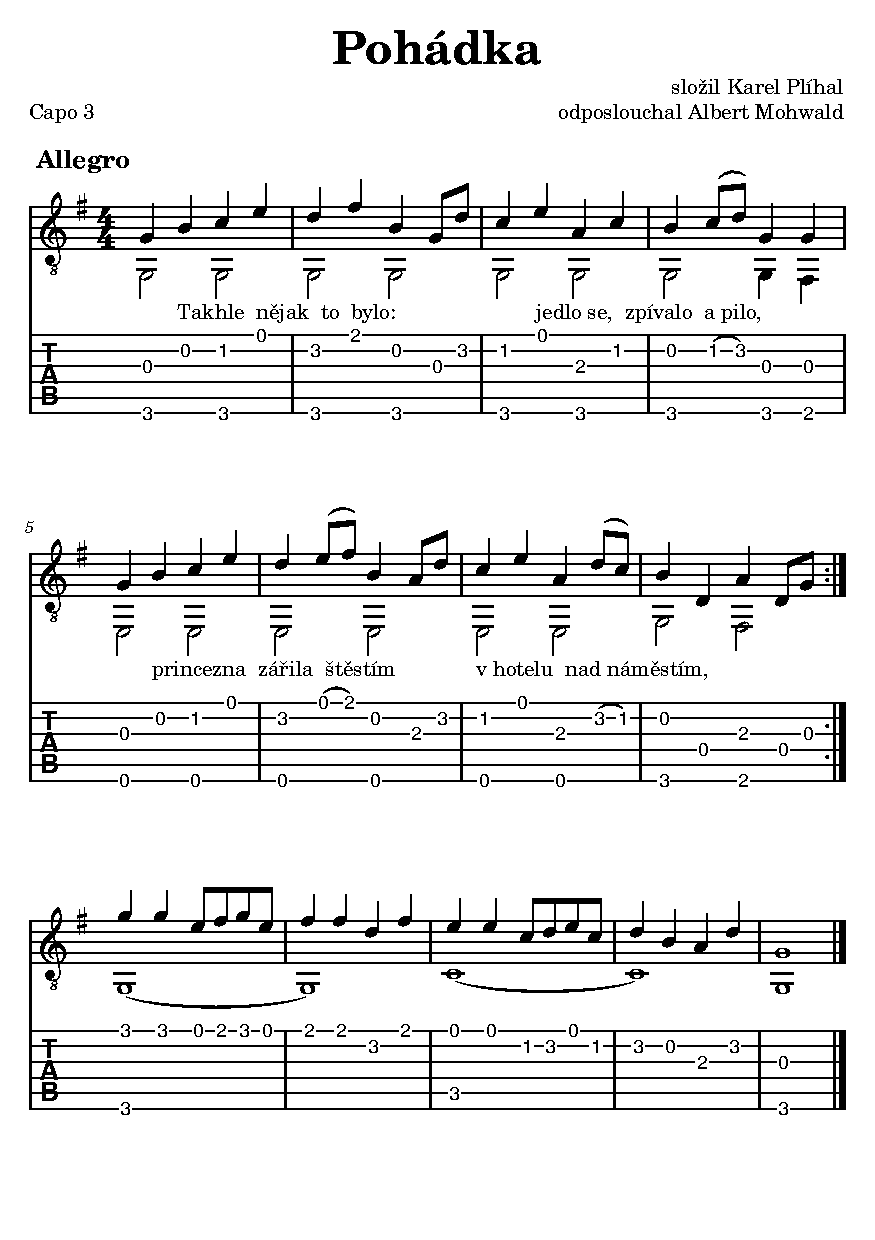
\includegraphics[scale=1.1]{../taby/pohadka-komplet.pdf}

\setcounter{Slokočet}{0}
\end{song}

\end{document}
